\documentclass[12pt]{letter}
\usepackage{amssymb,epsfig,amsmath,graphics,setspace,times,anysize}
\marginsize{1in}{1in}{-.5in}{.5in}

\newcommand{\note}[1]{{\color{blue}\footnote{\color{blue}  #1 }}}
\newcommand{\bs}[1]{\boldsymbol{#1}}
\newcommand{\mc}[1]{\mathcal{#1}}
\newcommand{\mr}[1]{\mathrm{#1}}
\newcommand{\bm}[1]{\mathbf{#1}}

\begin{document}

\signature{
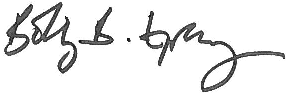
\includegraphics[scale=0.7,trim=10 0 0 50]{signature.png}\\
Robert B. Gramacy\\ {\it Professor of Statistics}\\ {\tt rbg@vt.edu}}
\name{Robert B. Gramacy}
\address{
Virginia Tech\\
Department of Statistics\\
250 Drillfield Dr.\\
Blacksburg, VA 24060\\
}


\begin{letter}{
Dan Jeske, {\em editor}\\
The American Statistician}


\includegraphics[width=2.5in,trim=0 0 0 0]{vt.png}

\opening{Dear Professor Jeske,}

I would like to submit the attached paper, ``A shiny update to an old
experiment game'' for possible publication in TAS.  
  
Last Fall I taught a graduate class at Virginia Tech on ``what Bobby likes to
do'' to help recruit research assistants.  (They made me call it ``Response
Surface Methods and Computer Experiments''.)  When preparing for the class I
found a pointer to a paper from the 1970s describing a computer game designed
to teach sequential design. I thought that a more modern version, using {\sf
R} and {\tt shiny} would be a fun way for the students to engage with similar,
but more state-of-the-art material.  It was super fun.  This paper outlines
the basic idea, and some details of the implementation that presented
``surprising challenges'' to me at the time---particularly to do with hosting a
dynamic interface in the cloud.  The biggest value may be in the supplementary
material which includes a full {\tt shiny} apps implementation, homeworks and
solutions in {\tt Rmarkdown}, and more.  These resources make the barriers to
reproduction or slight modification of the game quite low. Although my
material was targeted at a graduate student audience, slight tweaks could make
it appropriate for a less mature audience. I really think it's fun for all
ages!
     
Thank you for taking the time to consider this work. I hope that this
paper is of interest and up to the standards of TAS, and I look
forward to hearing your comments.

\vskip .5cm
\closing{Best regards,}
\end{letter}



\end{document}

